\documentclass[journal, a4paper]{IEEEtran}

% some very useful LaTeX packages include:

\usepackage{ctex}
\usepackage{graphicx}
\usepackage{animate}
\usepackage{subfigure}
\usepackage{url}
\usepackage{amssymb}
\usepackage{amsmath}
\usepackage{cite}
\usepackage{multirow}
\usepackage{listings}
\usepackage{booktabs}
\usepackage[colorlinks,linkcolor=blue]{hyperref}
\usepackage{listings}
\usepackage{xcolor}
\usepackage{float}
\usepackage{hyperref}
\usepackage{caption}
\usepackage{listings}
\usepackage{subfigure}
\usepackage{stfloats}

\lstset{
    columns=fixed,
    frame=none,
    keywordstyle=\color[RGB]{40,40,255},
    numberstyle=\footnotesize\color{darkgray},
    commentstyle=\it\color[RGB]{0,96,96},
    stringstyle=\rmfamily\slshape\color[RGB]{128,0,0},
    showstringspaces=false,
    tabsize=4
}

% Your document starts here!
\begin{document}

% Define document title and author
	\title{\textbf{黑盒白盒对抗攻击初探}}
    \author{李锦韬 2201213292 lijintao@stu.pku.edu.cn}
	\markboth{Principle and Application of big data Analysis in Python}{}
	\maketitle

% Main Part
\section{\textbf{问题背景}}
\label{section:adversarial attack}

对抗攻击是一种发生在深度学习模型推理阶段的攻击行为。在图像领域,对抗攻击通过扰动原本的图像数据,即在仅对图像进行非常小的修改的条件下,使得模型产生和原输出不同的输出结果。这种扰动,一般情况下是人类难以发觉的,甚至是肉眼无法分辨的。对抗攻击所产生的样本,一般具有如下特征:

\begin{itemize}
    \item 与原数据相比,变化极小
    \item 扰动会被人眼视为噪声,甚至人眼不可见
    \item 引起模型输出错误,但不会使得人类犯错
\end{itemize}

对抗攻击一般有两种场景:白盒和黑盒。

在\textbf{白盒攻击}的场景下,攻击者可以完全获取目标模型的结构、参数、训练数据等先验知识,并能够利用这些先验知识求解目标模型的梯度信息,以指导对抗样本的生成。即模型的所有参数和超参数都可见,允许使用``predict''和``gradient''接口。``predict''接口与黑盒攻击中相同;``gradient''接口,允许输入图像数据和期望的输出,计算任意层上的(包括输入数据上的)的梯度并返回。禁止训练和直接给权重赋值的操作。

在\textbf{黑盒攻击}的场景下,整个待攻击模型都处于黑盒中,其模型框架、模型结构等所有超参数,以及模型各层权重等参数均不可知,仅有一个``predict''接口可用。该接口允许输入图像数据,并返回模型输出的各个类别的概率。除此之外的所有操作均被禁止。

一般而言,图像模型的白盒攻击非常简单,因为输入数据上的梯度可以明确指出扰动的方向;而黑盒攻击相对困难,因为需要随机尝试扰动的方向。

在现实场景中,黑盒攻击占据大部分,因而仅仅在``攻击''这一层面上,黑盒攻击更为重要(例如攻击某个加密系统中的人脸识别系统或者虹膜识别系统)。但是,白盒攻击可以针对模型产生特定的样本,这些对抗样本可以被用来修复模型原本的缺陷。就像``黑客''和``白客'',白盒攻击的目的并不是为了攻破模型,而是发现模型的缺陷,并辅助修复,因此在``防御''的层面上,白盒攻击更有意义。

\subsection{白盒攻击(White-Box Attack)}
\label{section:adversarial attack;subsection:white-box}

分类器$C$接受输入图像$x$后产生概率向量$\hat y$(每一维对应一类),损失函数$L(x,y|C)$表示$\hat y=C(x)$与图像$x$的真实类别$y$的距离。$L(x,y|C)$越小说明$C$的预测与真实的类别越接近。在进行白盒攻击时,若我们期望分类器$C$给出的错误输出是$\tilde y$,则需要对$x$扰动得到$\tilde x$,并且使得$L(\tilde x,\tilde y|C)$尽量小。因此白盒攻击实质上是一个优化问题,即需要满足式\ref{equation:min},其中$D(a,b)$计算$a$和$b$的距离(例如欧氏距离)。式\ref{equation:min}表明,对抗样本$\tilde x$与原样本$x$被要求尽量相近,而$\tilde x$会使得模型$C$的输出为错误类别$\tilde y$。
\begin{align}
    &\min_{\tilde x} L(\tilde x,\tilde y|C)\ \&\ \min_{\tilde x} D(\tilde x, x) \label{equation:min}
\end{align}

一个最简单的白盒攻击算法就是梯度下降,即``固定模型调数据'':

\begin{itemize}
    \item 初始化样本,$x^{(0)}=x$;
    \item 计算样本梯度,需要使用反向传播算法;
\begin{equation}
    \nabla_{x^{(n)}}L(x^{(n)},\tilde y|C)=\frac{\partial L(x^{(n)},\tilde y|C)}{\partial x^{(n)}},\ n=0,1,2,\cdots \notag
\end{equation}
    \item 根据梯度扰动样本,$\alpha$为学习速率;
\begin{equation}
    x^{(n+1)}=x^{(n)}-\alpha\cdot\nabla_{x^{(n)}}L(x^{(n)},\tilde y|C),\ n=0,1,2,\cdots \notag
\end{equation}
    \item 重复迭代,直至收敛,返回$\tilde x=x^{(n)}$。
\begin{equation}
    arg\max C(x^{(n)})=arg\max \tilde y \label{equation:converge}
\end{equation}
\end{itemize}

\subsection{黑盒攻击(Black-Box Attack)}
\label{section:adversarial attack;subsection:black-box}

黑盒攻击的目标仍是解相同的优化问题,但是在求解过程中分类器$C$始终为黑盒,即不能计算任何梯度。因此在第\ref{section:adversarial attack;subsection:black-box}节提到的梯度下降的方法并不适用。

可以使用MCMC采样(Monte Carlo Markov chain sampling)进行黑盒攻击,MCMC采样可以被形象地理解为``走一步看一步'':

\begin{itemize}
    \item 初始化样本,$x^{(0)}=x$;
    \item 根据Markov转移概率$g(x|x^{(n)})$产生候选样本$x'$;
    \item 若$u\le C(x')[arg\max \tilde y]$,则拒绝$x'$,其中随机变量$u\sim U(0,1)$,$C(x')[arg\max \tilde y]$表示分类器在以$x'$为输入时,在目标类别上的预测概率;否则,接受$x'$;
    \item 若拒绝$x'$,则重新产生新的候选样本;否则,接受转移,$x^{(n+1)}=x'$;
    \item 重复迭代,直至收敛(满足式\ref{equation:converge}),返回$\tilde x=x^{(n)}$。
\end{itemize}

转移概率$g(x|x^{(n)})$基本可以任意指定(满足Markov链的遍历性和非周期性即可),例如可以指定$g(x|x^{(n)})$是以$x^{(n)}$为中心,以$\sigma^2$为方差的正态分布。需要说明的是,为了保证$\tilde x$和$x$尽量相近,我们可以设定迭代中单步扰动的变化阈值,一旦单步扰动的变化过大,则直接拒绝该候选样本,即若$D(x',x^{(n)})>\Delta_{max}$,则拒绝候选样本$x'$,其中$\Delta_{max}$为单步扰动的变化阈值。

\section{\textbf{数据集}}
\label{section:dataset}

此次作业项目使用Fashion MNIST数据集\footnote{数据集来源:\url{https://github.com/zalandoresearch/fashion-mnist}},其由60,000个样本的训练集和10,000个样本的测试集组成,每张图像的大小为28*28像素,均为灰度图像,内容实际上是10种不同类别的鞋帽服饰等产品平面图。

该数据集可以很方便地使用\verb|torchvision|框架中的\verb|datasets.FashionMNIST|类进行导入,因此本项目中不再额外保存数据文件。

\begin{figure}[H]\footnotesize
    \centering
    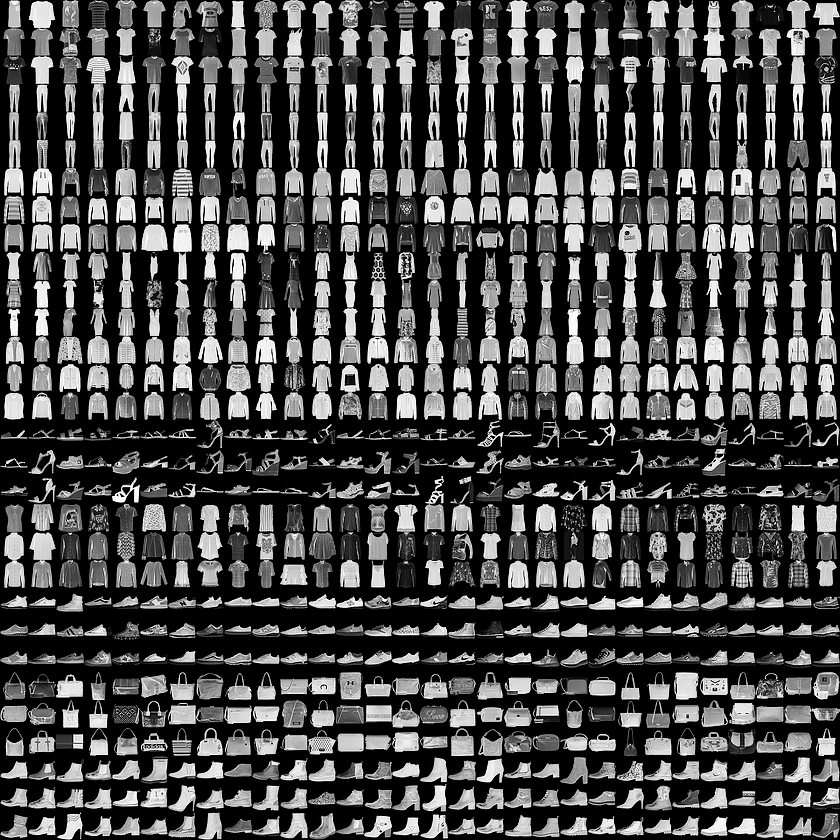
\includegraphics[width=\columnwidth]{../img/demo-fashion-mnist.png}\label{figure:demo fashion mnist}
    \captionsetup{font={small}}\caption{Fashion MNIST数据集示例}
    \label{figure:demo fashion mnist}
\end{figure}

\section{\textbf{项目实践}}
\label{section:experiment}

\subsection{训练分类模型}
\label{section:experiment;subsection:train model}

在基础图像分类模型上,本项目选择使用ResNet34结构,并使用PyTorch框架进行实现。在训练过程中,使用了交叉熵损失函数,选择使用Adam优化器,学习率设置为0.001,批次大小为128,训练轮数为40,学习率衰减参数为0.1,衰减间隔为10。

在训练过程中,使用了随机水平翻转、随机裁剪、随机擦除、标准化等数据预处理方法。分类器随着训练轮数的增加,分类精度和损失函数逐渐收敛,正如图\ref{figure:renet;figure:train-acc}和图\ref{figure:renet;figure:train-loss}所示,最终在测试集上的分类精度为93\%左右,在10个标签类别上的混淆矩阵如图\ref{figure:renet;figure:confused matrix}所示。

最终本项目使用的基础分类模型为第38个Epoch所对应的模型,其在测试集上的精度为93.71\%,模型文件为\verb|./model/checkpoint-60-93.71.pt|。

构建Fashion MNIST数据集基础分类器的代码参见\verb|./code/ResNet34.ipynb|。

\begin{figure*}[htbp] 
    \centering
    \subfigure[训练精度变化情况]{
        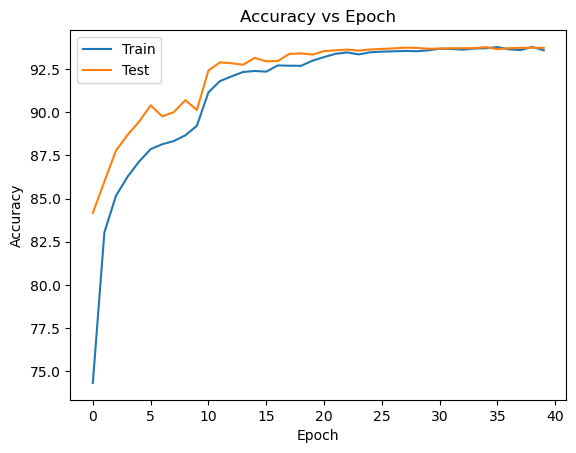
\includegraphics[width=0.65\columnwidth]{../img/ResNet.png}\label{figure:renet;figure:train-acc}}
    \subfigure[训练损失变化情况]{
        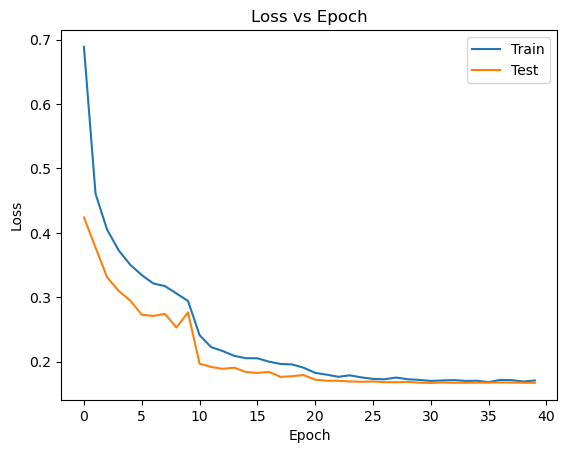
\includegraphics[width=0.65\columnwidth]{../img/ResNet-old-loss.png}\label{figure:renet;figure:train-loss}}
    \subfigure[混淆矩阵]{
        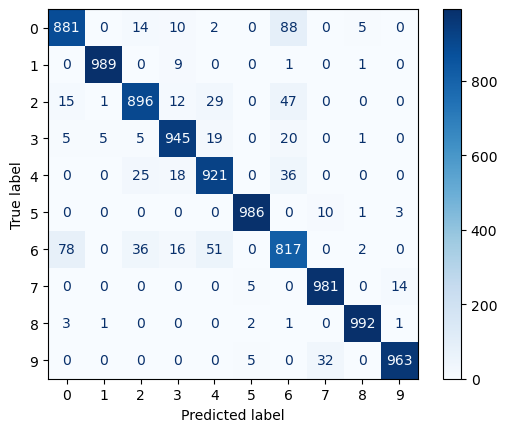
\includegraphics[width=0.65\columnwidth]{../img/ResNet-confused-matrix.png}\label{figure:renet;figure:confused matrix}}
    \captionsetup{font={small}}\caption{训练基础分类模型}\label{figure:resnet}
\end{figure*}

\subsection{白盒攻击}
\label{section:experiment;subsection:white-box attack}

对第\ref{section:experiment;subsection:train model}节中训练构建的模型进行\textbf{定向白盒攻击},即原本被正确分类的图像,在扰动后被判别为指定类别,原类别与目标类别一一对应,如表\ref{table:label}所示。

\begin{table}[h]\small
    \centering
    \begin{tabular}{lcccccccccc}
    \toprule
原正确类别 & 0 & 1 & 2 & 3 & 4 & 5 & 6 & 7 & 8 & 9 \\ 
    \midrule
指定的目标类别 & 1 & 2 & 3 & 4 & 5 & 6 & 7 & 8 & 9 & 0 \\
    \bottomrule
    \end{tabular}
    \captionsetup{font={small}}\caption{原正确类别与目标类别的对应关系}
    \label{table:label}
\end{table}

本项目中的白盒攻击算法采用定向的I-FGSM。该算法相当于使用迭代的FGSM,逐步修改测试图像,根据当前图像和目标类别之间的梯度,每次给图像变动 $\varepsilon \times \mathrm{Sign}\left( \nabla_{x^{(n)}}\left({x}^{(n)}, \hat{y} | C \right) \right)$ ,其中$\epsilon$为参数。由于是定向攻击,给图像施加的扰动方向应该是梯度的反方向。

本项目定义的攻击成功率计算方式为:基于I-FGSM算法,在迭代100次以内,扰动后的测试图像被分类器判断为目标类别的数量占所有被分类器正确分类的测试图像的比例。

I-FGSM算法中的$\epsilon$是超参数,需要通过搜索或试验的方式确定最优值。因此,本项目实验了许多不同的$\epsilon$取值,首先选择在$[.01, .02, .03, .1, .2, .25, .3, .5]$较大尺度上探索,确定攻击成功率随 $\epsilon$ 的大致分布情况,之后进一步在 $[.001, .002, .003, .004, .005, .006, .007, .008, .009]$ 细尺度小区间上进行了更局部的实验。

值得注意的是,在不定向攻击中,往往 $\epsilon$ 取值越大,攻击成功率越高,但在定向攻击中,$\epsilon$ 取值过大时,会导致图像变化过大,攻击成功率反而会下降,本项目实验的是定向攻击。超参数变化的相应规律正如图\ref{figure:White-Attack}所示,其显示了在测试集中分类正确图像上开展的$\epsilon$取值与所对应攻击成功率的相关情况。

经过实验,项目最终确定 $\epsilon=0.02$ 时,所带来的图像变化较少,攻击成功率也最高,达到 $14.37\%$ 。

\begin{figure}[t] 
    \centering
    \subfigure[细粒度小尺度]{
        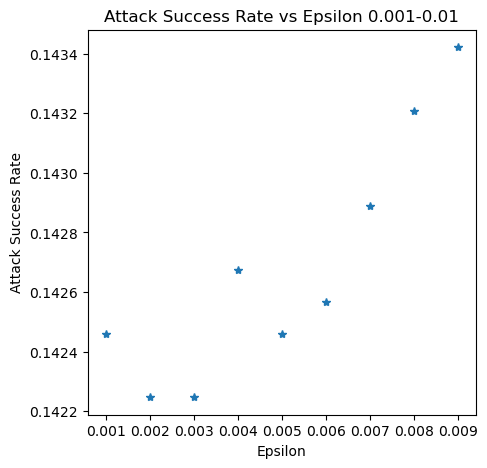
\includegraphics[width=0.45\columnwidth]{../img/White Attack Success Rate vs Epsilon 0.001-0.01.png}}
    \subfigure[粗粒度大尺度]{
        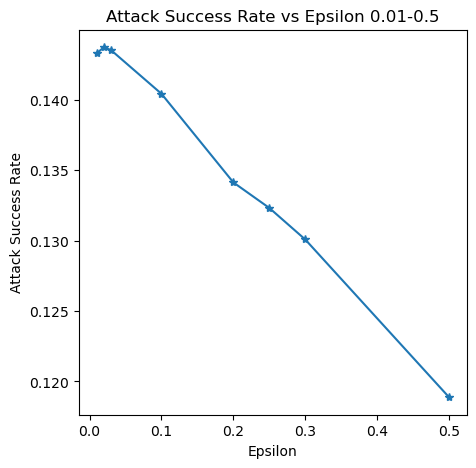
\includegraphics[width=0.44\columnwidth]{../img/White Attack Success Rate vs Epsilon 0.01-0.5.png}}
    \captionsetup{font={small}}\caption{实验寻找最佳$\epsilon$}\label{figure:White-Attack}
\end{figure}

图\ref{figure:White-Attack-Sample}为部分攻击成功的样本图片,图片两两一组,左侧的为原始图像,右侧的为白盒攻击图像。可见 $\epsilon$ 取 $0.02$ 时白盒攻击对图像的改动很微小,而且主要体现为图像亮度/对比度的变化,或改变图像上部分区域的纹理强度,使得分类器模型错判。例如在运动鞋$\to$袋子的定向攻击上,白盒攻击消除了鞋子的部分局部纹理特征,使分类器失效。

\begin{figure}[t] 
    \centering
        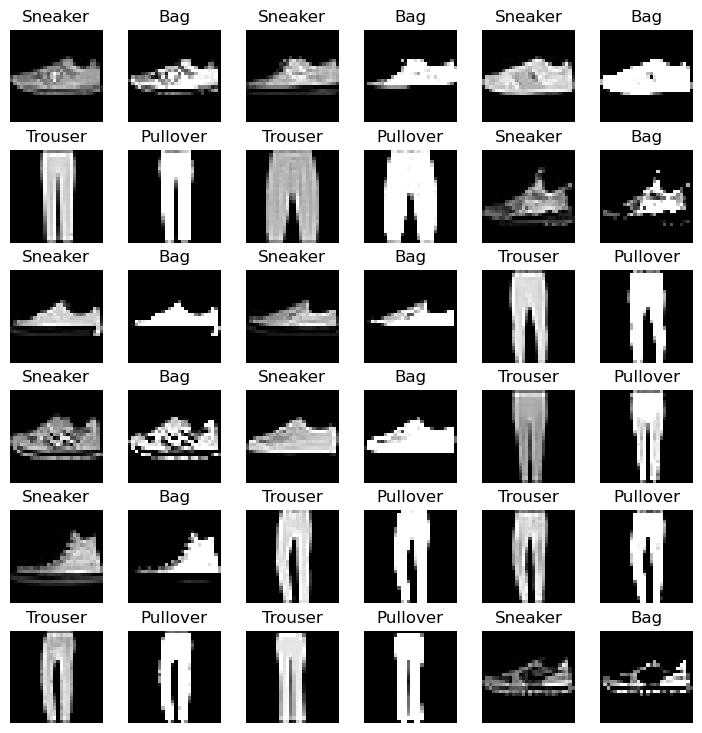
\includegraphics[width=\columnwidth]{../img/white-attack-sample1.png}
    \captionsetup{font={small}}\caption{白盒攻击得到的部分对抗样本}\label{figure:White-Attack-Sample}
\end{figure}

以上对构建的分类器进行定向白盒攻击的相关代码参见\verb|./code/white-attack.ipynb|,对分类器进行不定向白盒攻击时的超参数规律变化本项目也做了尝试,相关代码参见\verb|./code/white-nodir.ipynb|。

\subsection{黑盒攻击}
\label{section:requirement;subsection:black-box attack}

对第\ref{section:experiment;subsection:train model}节中训练构建的模型进行\textbf{定向黑盒攻击},原类别与目标类别的对应关系如表\ref{table:label}所示。本项目选择的黑盒攻击的算法为MCMC采样,其可以直接产生对抗样本进行攻击。

MCMC采样算法每次在图像上施加正态扰动,迭代进行直到分类器将图像分错成攻击目标类别,具体算法流程可见第\ref{section:adversarial attack;subsection:black-box}节。由于MCMC采样的耗时较长,本项目选择随机抽取了1500个分类器可以正确分类的测试集样本进行测试。在每次迭代中,单张图像攻击MCMC采样循环最高限制在300次,每次施加的扰动符合以原图为中心的正态分布,其分布的标准差为 $0.03$ (数据输入前经过标准化,大约相当于灰度值7以内),使用 $f1-\mathrm{Loss}<0.05$ 限制扰动前后的图像变化差距,在以上迭代限制条件内能够使得分类器定向错分即视为攻击成功,相应的可计算出攻击成功率。

\begin{figure}[!t]
    \centering
        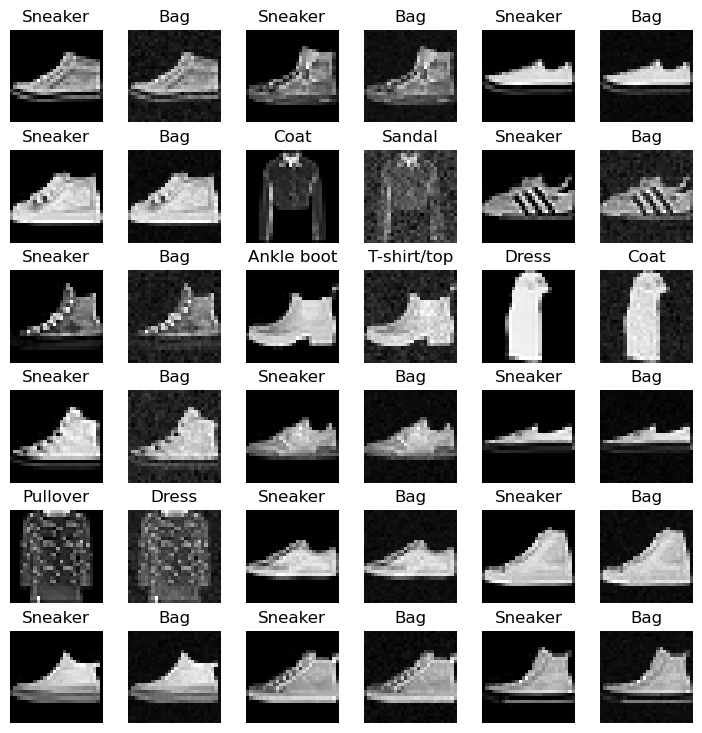
\includegraphics[width=\columnwidth]{../img/black-attack-sample4.png}
    \captionsetup{font={small}}\caption{黑盒攻击得到的部分对抗样本}\label{figure:Black-Attack-Sample}
\end{figure}

最终MCMC采样黑盒攻击算法对本项目构建的分类器的攻击成功率为 $9.73\%$,比定向白盒攻击的攻击成功率低了4.64\%,说明在缺少模型知识时想要对分类器进行攻击相对困难了一些,但近10\%的攻击成功率说明原模型的稳健型不是非常理想。由此也能体会到对抗攻击现象给深度学习模型的安全应用带来的严峻挑战,这值得我们进一步关注关注和深入研究。

图\ref{figure:Black-Attack-Sample}为部分成功进行MCMC采样黑盒攻击得到的对抗样本,其同样是两两一组,左侧的为原始图像,右侧的为黑盒攻击图像。可见MCMC采样算法对样本原图像的改动不大,在视觉上看来像是给图像增加了部分随机(在模型看来可能是定向的)噪声。

以上对构建的分类器进行定向黑盒攻击的相关代码参见\verb|./code/black-attack.ipynb|。

\section{\textbf{总结}}

本项目使用开源的Fashion MNIST数据集,基于ResNet34网络构建了一个图像分类器,其在测试集上的准确率为93.71\%。

项目针对所构建的分类器进行了定向白盒攻击和定向黑盒攻击,算法分别采用I-FGSM和MCMC采样,对应的攻击成功率分别为 $14.37\%$ 和 $9.73\%$。对比两种攻击算法,I-FGSM算法的攻击成功率更高,因为其直接可以获取模型的梯度信息,模型对其而言是完全透明的,但即使超参数$\epsilon$选取的非常小,相比较而言其对图像的改动比较明显,根据项目设置的攻击方向,主要体现为亮度和对比度的变换、涂抹消除局部纹理等。而MCMC采样算法的攻击成功率较低,但其对图像的改动更小,主要体现为给图像加上了一定的高斯随机噪声,对防范实践中的模型对抗攻击意义更大。

\section*{\textbf{项目文件构成说明}}

\begin{itemize}
    \item \verb|./code/|:存放项目代码,包括模型训练、黑白盒对抗攻击、尝试不同的超参数和数据预处理方式训练分类器、尝试不定向白盒攻击等代码。
    \item \verb|./img/|:存放项目图片,包括项目报告中的图片、对抗攻击得到的部分对抗样本等。
    \item \verb|./model|:存放项目模型,包括对抗攻击中使用的分类器模型(GitHub仓库没有存储)。
    \item \verb|./report/|:项目报告,包括本项目的 \LaTeX 源码与对应的PDF文档。
    \item 本项目使用Git进行版本管理,所有源码位于:\url{https://github.com/AkexStar/LearnPython/tree/main/final}
    
\end{itemize}
% Your document ends here!
\end{document}